\documentclass[a4paper,11pt]{article}
\usepackage{amsthm}
\usepackage{amssymb}
\usepackage{color}
\usepackage{graphicx}
\usepackage{float}
\usepackage{fullpage}
\usepackage{verbatim}
\usepackage{tikz}
\usetikzlibrary{arrows}
\newtheorem{theorem}{Theorem}
\newtheorem{lemma}{Lemma}
\newtheorem*{remark}{Remark}

       % define the title
       \title{9. Extracting Weather and Sentiment from Tweets}
       \begin{document}
       % generates the title
       \maketitle

\section{Introduction}
There are approximately 200 million active users on Twitter and 400 million tweets are posted on a daily basis. We can leverage these tweets about everyday topics to learn machine learning methods and keywords that best process a tweet's intent and sentiment. With that in mind, the specific domain of weather is particularly rich data set to begin our study– weather is a common topic of conversation, and this is no different in the Twitter sphere. With twitter as an individual's outlet, he can express his joy about the sun, complain about overbearing heat, or talk about the upcoming forecast. We aim to build a classifier than can extract a tweet's sentiment, time frame, and weather condition of tweets given prior data. Then we can examine our classifier to determine which algorithms are most effective and which words are the best indicators.

To answer our questions, we applied different learning methods on weather related tweets. Our findings showed that Suppport Vector Machines and Naive Bayes were accurate classifiers to extract weather information from a tweet. In addition, we discovered a few keywords in a tweet were the best indicators, while the rest of the words had a little or no effect on a tweet's sentiment, timeframe, and weather condition. Finally, we created a Markov Random Field classifier that used a tweet's relative timeframe and location to predict a tweet's message.


\section{Problem Definition and Methods}
\subsection{Task Definition}
	Through our project, which was one of the Kaggle Projects assigned, we aimed to calculate classification probabilities for incoming tweets into 24 labels. These 24 labels came from 3 main categories:

\begin{itemize}
\item Sentiment = \{Can’t tell, Positive, Neutral, Negative, Unrelated to weather\}
\item When = \{Current, Future, Can’t tell, Past\}
\item Kind = \{Clouds, Cold, Dry, Hot, Humid, Hurricane, Can’t tell, Ice, Other, Rain, Snow, Storms, Sun, Tornado, Wind\}
\end{itemize}

	Our task was to take an incoming tweet and classify it to produce a vector of 24 confidence scores: one for each label. This confidence score indicated a level of confidence for that particular tweet to have significant information about that particular label. The categories of Sentiment and When could only have one classification with a positive confidence score (as for instance, a weather related event cannot happen in the past as well as in the future), but there could be multiple positive confidence scores for labels in the Kind category (it can be ``cloudy'' as well as ``rainy'' at the same time). Our training set contained tweets, locations, and a confidence score for each of the 24 possible labels. 

	For each tweet, we would like to have definitive ``sentiment'', ``when'', and ``kind'' values 

\subsection{Algorithm}
	Given our input training sets (Kaggle and Cheng-Caverlee-Lee) and constraints, we decided to use a set of algorithms that we felt would best classify our data. The categories of Sentiment and When were discriminative in nature and therefore merited the use of discriminative algorithms, whereas the Kind category was generative (requiring a real-valued number representing a ``score'' of how likely that kind of weather was, given the tweet. A single tweet could thus have multiple kinds of weather at once. Thus the algorithms we ended up using were:

\begin{enumerate}
\item Support Vector Machine

We converted our input dataset to the Svmlight format and used Professor Joachims’s Svmlight module to learn and classify each of the 24 separate labels as binary classifiers. We then took the max of the resulting margins within the categories to single out the “best” labels.

\item Decision Tree

We used the TDIDT ID3 algorithm to build Decision Tree classifiers for each of the 24 labels, with splitting criteria $\ge 1$ and $\ge 0$. We then took the max of the resulting classifications to similarly decide on the “best” labels.

\item Naïve Bayes

We used independent class conditional probabilities of each significant word (or combination of words) in the tweet, and used that to calculate the probability of a label being assigned to a tweet.

\item Markov Random Field

	As an effort to make Naive Bayes less ``naive'', we introduced conditional dependencies (based on the location and timestamp of a tweet) to classify incoming test tweets better. This was based on the assumption that tweets in nearby locations and within the same intervals of time, would have some level of similarity when it comes to the kind of weather they would be talking about. Therefore, our MRF classifier made the use of these dependencies to classify incoming tweets based on previous tweets, weighing ``similar'' tweets greater than ``dissimilar'' ones when making a classification.
\end{enumerate}

	Each of these algorithms, along with the constraints we put on them, are explained in more detail further sections.



\section{Methodology}
\subsection{Data Manipulation}
\subsubsection{Preprocessing}
	The provided Kaggle data comes with a guarantee that the tweets are either about weather or are labelled in a way that indicates that they aren't about weather. So, there was no need to filter out entired tweets. But, as expected, a lot of the content of tweets aren't particularly important to our analysis. Stopwords like ``a'' and ``the'' are not worth considering in our algorithms. Using a predefined list of stopwords (reference mentioned in Appendix), we filtered out all stopwords from tweets. Moreover, we filtered out some common Twitter-specific jargon that bears no meaning in our problem, e.g. ``RT'' and ``@mention''.
	
	 Although capitalization may be indicative of strong emotions (and therefore helpful to sentiment), we've chosen to focus on the words themselves, so all words in each tweet are converted to lowercase. Lastly, all  punctuation symbols within a tweet are removed. Well, not quite \emph{all} punctuation...emoticons are comprised of punctuation marks and can be quite useful with regards to understanding sentiment, so all emoticons are kept in the tweets and treated as any other word.



\subsubsection{Important Words}
	The discriminative algorithms we use (SVM and decision trees) rely on translating our tweets into feature vectors, where each feature is a word of the vocabulary. Our vocabulary $V$ was very large (on the order of $10^7$), so it would be unwieldy to represent each tweet with a vector of length $|V|$, especially since some words aren't as important as others in determining weather/sentiment from tweets. To deal with this issue, we used class conditional probabilities from Naive Bayes (algorithm discussed later) to determine which words are most important in determining sentiment, when, and kind -- the notion of ``most important'' has to do with which words have a high probability of occuring given that, for example, the kind of weather is ``rainy''.

	The most important words for sentiment, when, and kind generated from this analysis are depicted in the below word clouds (larger words are more important than smaller ones). As we can see, most of these important words are indeed related to weather. For instance, it is unsurprising that the word ``good'' has high importance for sentiment, and ``storm'' has high importance for kind.

\begin{figure}[!htb]
\minipage{0.5\textwidth}
  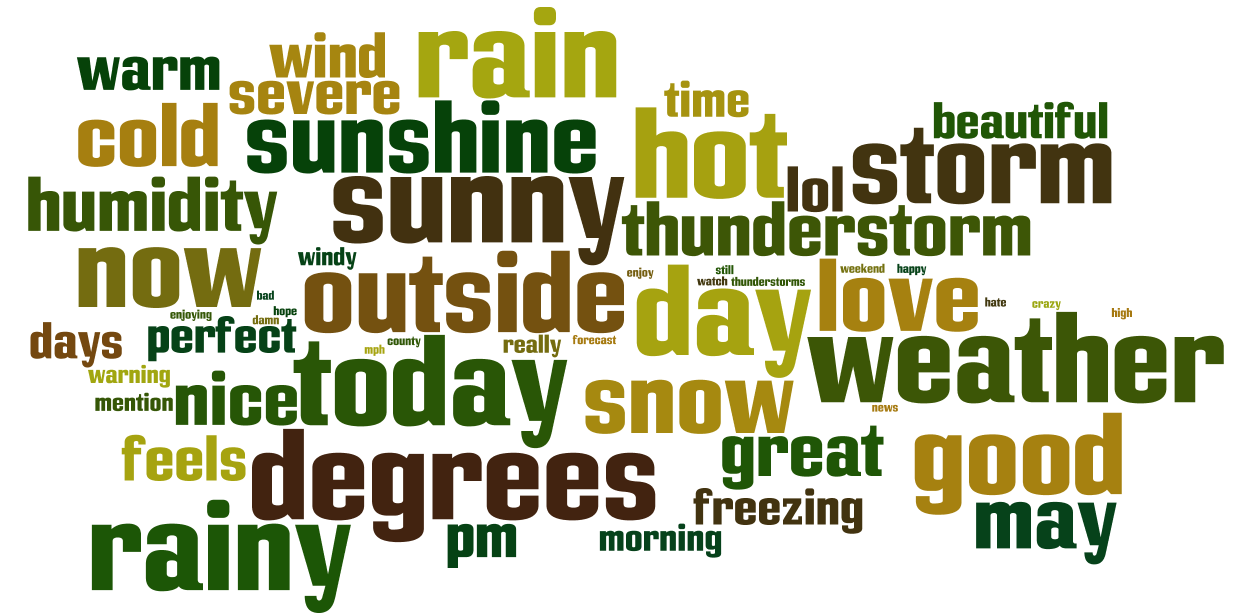
\includegraphics[width=\linewidth]{wordclouds/31sentiment}
  \caption{Top 30 ``sentiment'' words}\label{fig:awesome_image1}
\endminipage\hfill
\minipage{0.5\textwidth}
  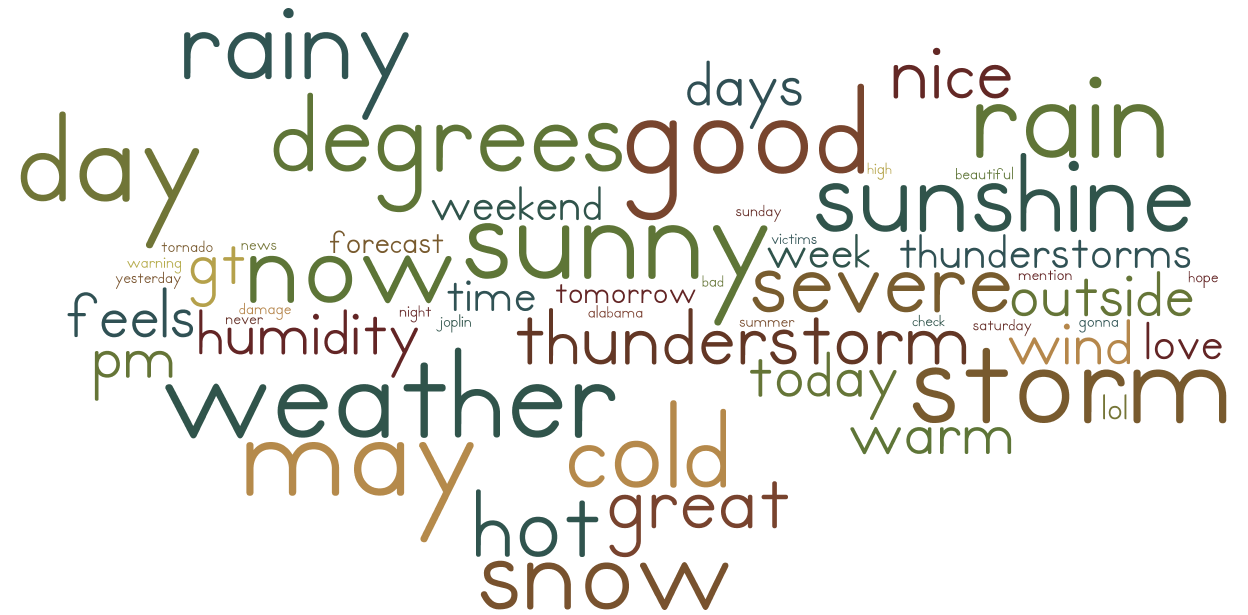
\includegraphics[width=\linewidth]{wordclouds/31when}
  \caption{Top 30 ``when'' words}\label{fig:awesome_image2}
\endminipage\hfill
\noindent\makebox[\textwidth][c]{%
\minipage{0.5\textwidth}%
  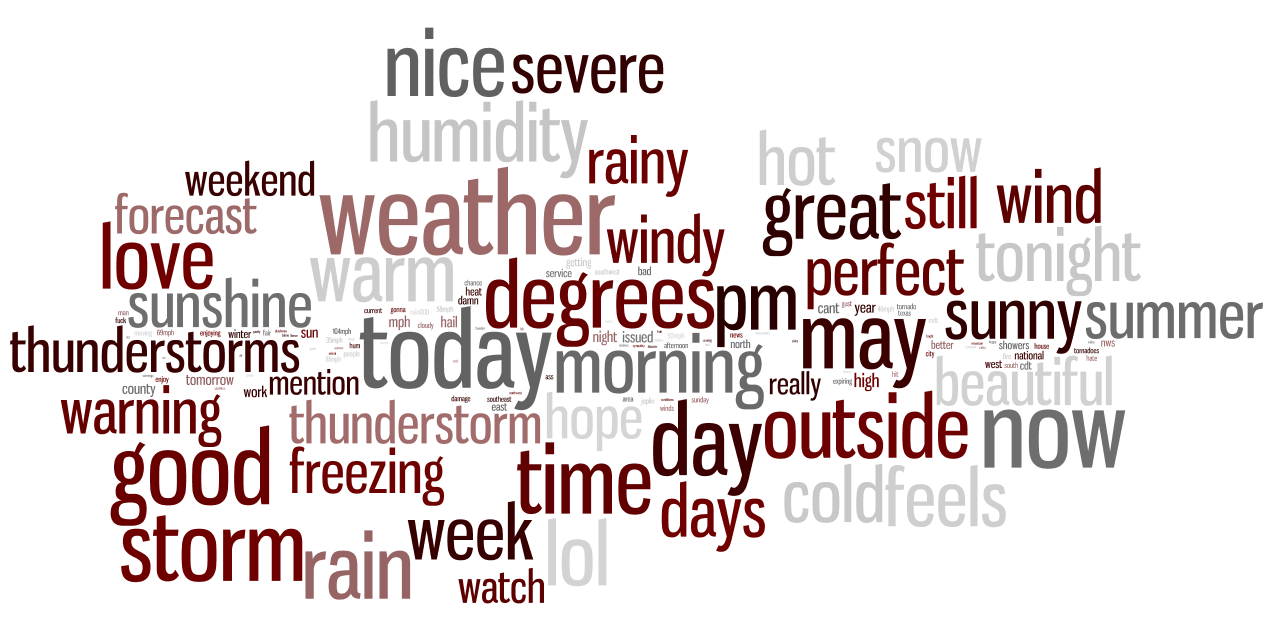
\includegraphics[width=\linewidth]{wordclouds/50kindwords}
  \caption{Top 50 ``kind'' words}\label{fig:awesome_image3}
\endminipage}
\end{figure}


\subsubsection{Data for MRF}
	We explore a method for tackling this problem using Markov Random Fields (MRF), which relies on location data and time data. The available Kaggle data doesn't have timestamps, so we utilized a separate dataset (referenced in Appendix). This data set is unlabelled and not weather-specific. To distill out the tweets related to weather, we removed all tweets that do not contain any words from the list of most important words for determining the kind of weather (gathering of important words discussed in previous subsection). The tweets were then labelled using decision trees (algorithm methodology discussed later), which did the best job of determining the kind of weather. Finally, we sent the remaining tweets through the same preprocessing specified in the ``Preprocessing'' subsection above.

\subsection{Preliminary Methods}
\subsubsection{Decision Trees}
	One discriminative algorithm we used to classify the tweets is decision trees. From the homework set, we saw that decision trees could be useful for classifying texts into different genres. Therefore, we used the TDIT algorithm along with information gain to the build decision trees for classifying the ``when'', ``sentiment'' and ``kind'' labels of tweets. Since a tweet can have multiple ``kind'' labels, we constructed a tree for each of the fifteen labels indicating either ``positive'' or ``negative.'' Then the vector of ``kind'' labels can be generated from the output of each of the fifteen trees.

	The feature vectors used to represent the tweets were the bag of ``important'' words constructed from the Naïve Bayes conditional probabilities. Thus, each attribute represented a word count. Then the splitting criteria used was either $>0$ or $>1$ depending on which gave more information gain. In order to prevent overfitting early stopping was used. Lastly, cross validation was used to determine the optimal tree depth from a range of 2 to 60. 

\subsubsection{SVM}
	The input dataset from Kaggle was converted into the Svmlight format, which included obtaining the ``best features'' that the Naïve Bayes algorithm produced as the ``important bag of words'', and creating the svmlight format from those particular word counts. We used Professor Joachims’s svmlight module executable to learn classifying models for each of the 24 labels, with varying c-values (to indicate the ``slack'' allowed for the classifier). 

	For each label, the best c-values (that produced the highest accuracy on the validation set) were used to prevent over-fitting in the final classifiers. These classifiers were inherently binary, and gave the geometric margin of a validation tweet from the separator. This geometric margin (normalized) was used to determine best the sentiment and when labels (by taking the max), and the best kind labels (those that were $\ge 0.7$).

\subsubsection{Naive Bayes}
	We use Naive Bayes to learn the ``sentiment'' and ``when'' labels of a tweet, and to learn which kinds of weather are occuring. In addition to implementing the off-the-shelf version of the algorithm learned in class, we also took steps to make Naive Bayes a little less naive.
	
	Traditionally, in this setting, Naive Bayes breaks a tweet up into words and maintains probabilities corresponding to each word. Our implementation of the algorithm allows support for maintaining probabilities corresponding to groups of $k$ words for any $k$. For instance, if the tweet is ``not sunny today :('', we add the pairs of words ``not sunny'', ``sunny today'', and ``today :('' to our vocabulary (i.e. we look at bigrams). The groups of words consist of consecutive words as in this example. We experimented with different blends of unigrams, bigrams, and trigrams when performing Naive Bayes.


\subsection{Advanced Methods}
\subsubsection{Markov Random Fields (MRF)}
	Although the words within a tweet can be strong indicators of the weather conditions surrounding a tweet, it is also helpful to know the location and time of the tweet. For example, if the tweet is made in Boston in December, there is likely to be snow. The traditional machine learning methods presented thus far don't leverage this sort of spatial and temporal data to make better-informed decisions. To this end, Markov Random Fields are particularly helpful.

	The data used for MRF was described in the ``Data manipulation'' section. With each tweet in this data set is information on the city from which the tweet's user came from\footnote{It could be the case that a user from city A is actually making a tweet from city B and commenting on city B's weather, but the hope is that this isn't too frequent.}, and to simplify our model we mapped each city to its state, just to make the locations less granular. 

	Now, the goal for us here is to try to use location/time data to extract the kind of weather condition from a tweet. The general idea behind Markov Random Fields is to model dependencies between variables and gain insight from these dependencies when making predictions. To use this concept, we assume that close-together regions experience similar weather, and we focus on just a small window of time (half a day) to avoid vast variations in weather within a region. 

	The graphical model is as follows. We have a graph with nodes corresponding to states within the United States. There is an undirected edge between nodes if the corresponding states share a border. For each edge $e=(u,v)$ we assign a $15 \times 15$ table $T_e$, where the rows and columns are the 15 different weather kind categories -- the rows correspond to state $u$ and the columns correspond to state $v$ (without loss of generality), and the value in table entry $T_e[i,j]$ is relatively large if there's a high likelihood of state $u$ experiencing weather $i$ when state $v$ experiences weather $j$, but relatively small if the likelihood of this is low. Given our assumption that neighboring states have similar weather, this means that values along the main diagonal will be larger than values off the main diagonal.

	The goal is to determine the kind of weather for each node (i.e. each window of time for each region), and then label each tweet from that location/time with the kind of weather for the corresponding node. So the question is, how does one label a node? Consider a node $u$ with, say, four neighbors $n_1, n_2, n_3, n_4$ which have already have labels $l_1, l_2, l_3,l_4$ fixed. We also already have a training set of tweets from the location/time corresponding to node $u$, and we collect the words from all these tweets into a bag of words; for each word, we have a length-15 vector $\bar{w}$ of probabilties $P(y|w)$, i.e. the probability that the kind of weather is $y$ (for all 15 kinds of weather) given that a tweet has word $w$. 

	Then, to label a node, we do the following. For each neighbor $n_i$ there is an edge matrix $T_{(n_i,u)}$ as defined earlier, and since the label of $n_i$ is fixed, we have a row vector (could be a column vector, but I'll call it a row without loss of generality) corresponding to the likelihood of $u$ having a certain label given that $n_i$ has label $l_i$. Let's normalize these vectors so that the entries are probabilities. 

	Additionally, for each tweet we're classifying from $u$'s location/time, we have a vector of probabilities that the tweet belongs to each kind of weather (from Naive Bayes). Multipliying these tweet vectors and neighbor vectors pointwise, and then normalizing, we produce a final vector $v$ of probabilities that node $u$ belongs to each particular kind of weather -- these probabilties therefore take into account the training data \emph{and} the location/time, as desired. Using this vector of probabilities, we draw at random a kind of weather to label $u$ with (the random drawing is done in a way so that the probability of drawing the $i^{th}$ kind is $v_i$).

	Repeating this process for each node gives us labels for each node. This begs the question -- how do we come up with an initial labelling of nodes? Certainly, some initial labelling is necessary in order to assume that the neighbors are pre-labelled. To this end, we require the method Gibbs Sampling. We assign each node an initial label at random (or not-so-random, e.g. an educated guess given prior results from Naive Bayes), and then perform our labelling as described. After several (perhaps hundreds) iterations of labelling each node, we'd converge to a label likely to be correct. At this point, we get a label $l$ for each location/time node $u$ by taking the mode of all labels produced for $u$ throughout the Gibbs Sampling, and we assign label $l$ to each tweet from the location/time corresponding to $u$. 

	One slight shortcoming here is that we assign each tweet one kind of weather, when a location can experience multiple kinds of weather at one (e.g. cloudiness and rain). A solution here is to look at the final probability vector for a node and label the node with the label of max probability plus all labels with probablilities greater than or equal to some threshold (e.g. 0.7).

\section{Experimental Evaluation}
\subsection{Results}
	To evaluate the performance of our algorithms we established a base line that predicts random labels for sentiment and kind, and for when we predicted everything as ``current'' time. The accuracy values for assigning these labels to the test set is shown below:

\begin{center}
When accuracy = 77.6\%, Sentiment accuracy  = 16.5\%, Kind Accuracy = 30.3\%
\end{center}

	We will compare these baseline accuracies to the accuracies of our learning algorithms to measure their performance. Note: the ``when'' baseline was determined by always guessing that the time frame was ``current time''. This means that 77.6\% of our tweets are about the current weather. 

\subsubsection{Decision Trees}
	Decision trees performed relatively well and produced reasonable accuracies for the three different categories. The graph below shows the accuracy values against varying tree height for the ``when'' and ``sentiment'' labels. Based on the graph, there does not appear to be dramatic changes in accuracy with varying tree height, however we can see the overfitting and underfitting portions of the graph. 

%DECISION TREE ACCURACY VS TREE DEPTH
\begin{figure}[H]
\noindent\makebox[\textwidth][c]{%
\minipage{0.65\textwidth}%
  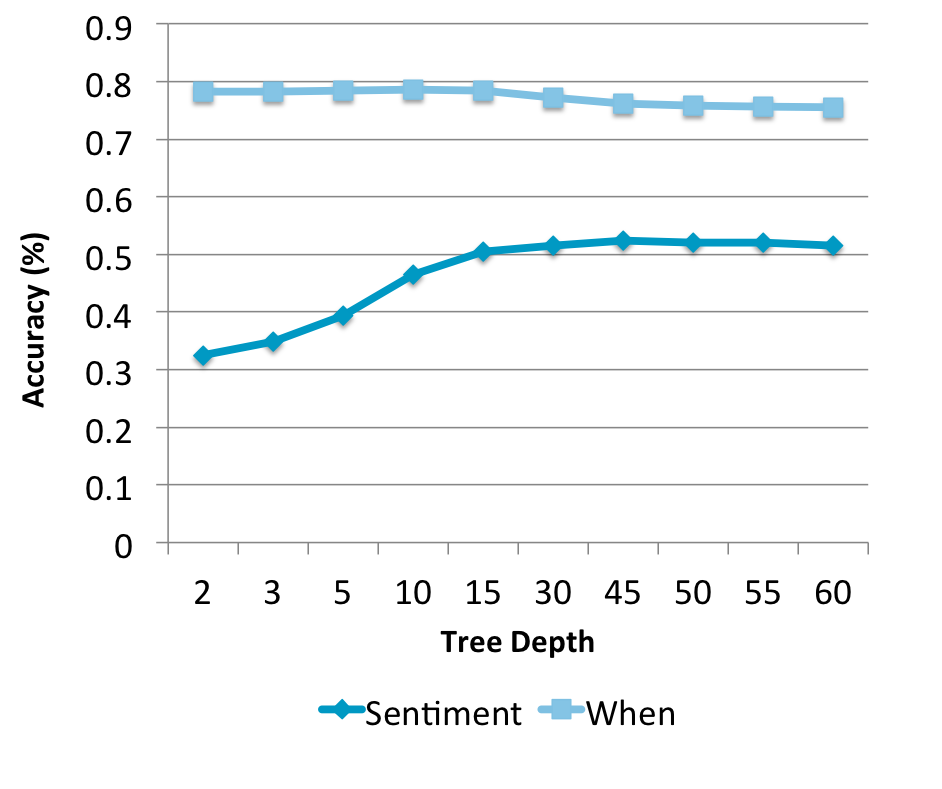
\includegraphics[width=\linewidth]{results/decision}
  \caption{Accuracy vs. Tree Depth}\label{fig:decision}
\endminipage}
\end{figure}

	The optimal height for the ``when'' label is 10 while the optimal height for the ``sentiment'' label is 45. This implies that the decision tree requires much more information to predict the sentiment of a tweet as oppose to the time frame of a tweet. Also, the decision tree was able to predict the ``when'' label of a tweet with a much higher accuracy of 78.6\%, while only a 52.9\% accuracy for the ``sentiment'' label. However, the baseline for the ``when'' label was 76.7\%, so the accuracy for the decision tree is not much higher. This indicates that the decision tree was not very effective in classifying the time frame of a tweet. Since, the baseline for ``when'' is already so high, it is hard to create a classifier that performs significantly better.   

            The decision tree models performed very well for the weather ``kind'' label. As mentioned earlier, multiple trees were used to classify either ``positive'' or ``negative'' for each of the different kinds of weather. All fifteen decision trees with a height of 30 produced accuracies above 95\%. This seems fairly high, but it is plausible because the presences of key words is the strongest indicator of the ``kind'' of weather in a tweet. For example, the word at the root node for each the decision trees has been the type of weather itself. For example the root node for the decision tree classifying whether a tweet is about cold weather is the word ``cold.'' 

	Another reason for the high accuracies values may be due to the change from confidence scores to binary values. We stated earlier that confidence scores above 0.7 are considered positive and confidence scores below 0.3 are considered negative. This means that only tweets that are clearly about a certain type of weather will be classified as either positive or negative. Thus, these are the tweets that explicitly say what the weather is by using descriptive words. However, by doing this we may be ignoring tweets where the weather can be inferred from the meaning behind the texts. These are the tweets that the decision trees may not perform as well on because it cannot rely solely on the presence of key words. Thus, the accuracy values may be lower if we changed the threshold on the confidence scores. 

\subsubsection{Support Vector Machines}

The input dataset from Kaggle was converted into the Svmlight format, which included obtaining the ``best features'' that the Naïve Bayes algorithm produced as the ``important bag of words'', and creating the svmlight format from those particular word counts. We used Professor Joachims’s svmlight module executable to learn classifying models for each of the 24 labels, with varying c-values (to indicate the ``slack'' allowed for the classifier). For each label, the best c-values (that produced the highest accuracy on the validation set) were used to prevent over-fitting in the final classifiers. These classifiers were inherently binary, and gave the geometric margin of a validation tweet from the separator. This geometric margin (normalized) was used to determine best the sentiment and when labels (by taking the max), and the best kind labels (those that were >= 0.7).
 
 
The SVM classifiers performed pretty well on the training set as binary classifiers. Each of the three different categories responded differently to the SVM classifiers. The ``sentiment'' classifier was the weakest of the three, as there is always an ambiguity when it comes to ``sentiment''. Certain words can classify as positive sentiment for a few people and negative sentiment for a few others. ``Rain'' is a good example of such a dichotomy. A difference in positive outlook among people in different parts of the country (or at different times of the day) also affects the ``sentiment'' classifier. A low accuracy of 63.15% characterizes this ambiguity.
 
The ``when'' and ``kind'' classifiers performed extremely well with average accuracies of 79.67\% and 97.77\%. This makes sense because the ``when'' and “kind” classifiers have very high class-conditional probabilities with certain words. For instance, the word ``was'' in a tweet (or similar words indicating grammatical past tense), will give a classification of “past” with a very high probability. Similarly for the``kind'' classifier, words related to the weather are few and extremely specific.
 
The binary classifiers and their accuracy values (and precision/recall for ``kind'') are given as follows:

%SVM ACCURACY CHARTS
\begin{figure}[H]
\minipage{0.45\textwidth}
  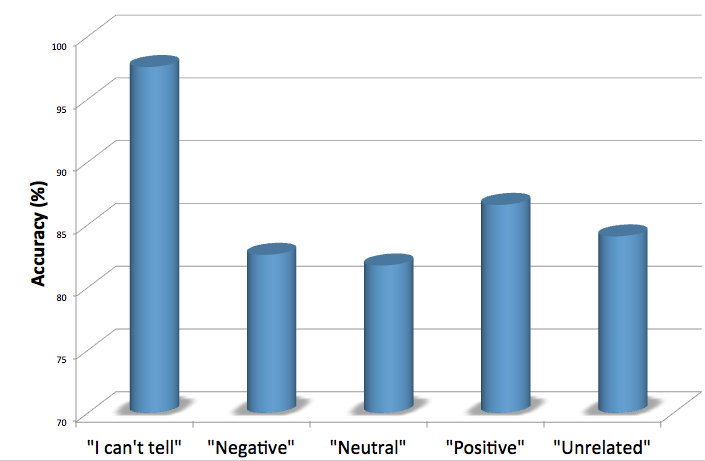
\includegraphics[width=\linewidth]{results/svmSentiment}
  \caption{``Sentiment'' Accuracy}\label{fig:svmSentiment}
\endminipage\hfill
\minipage{0.45\textwidth}
  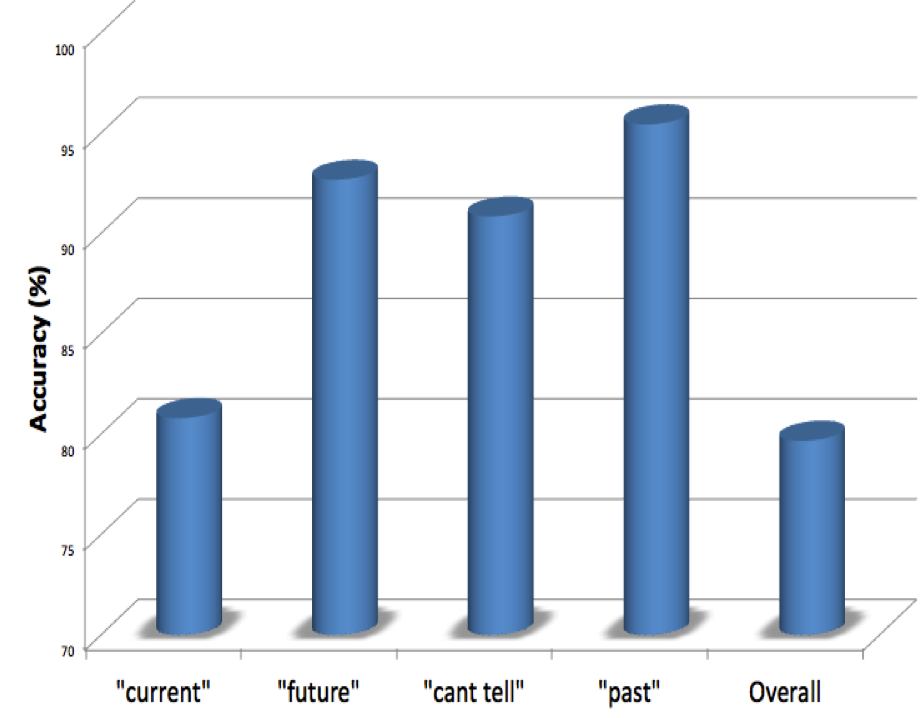
\includegraphics[width=\linewidth]{results/svmWhen}
  \caption{``When'' Accuracy}\label{fig:svmWhen}
\endminipage\hfill
\minipage{0.75\textwidth}%
  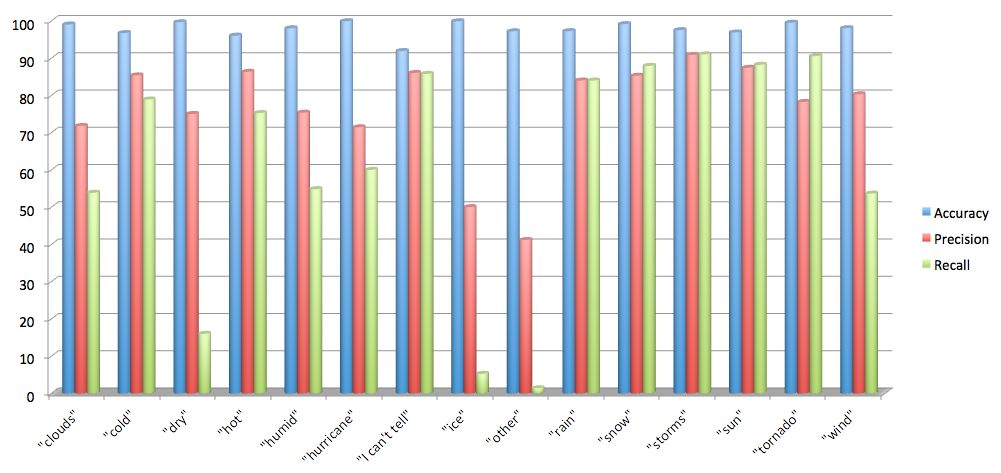
\includegraphics[width=\linewidth]{results/svmKind}
  \caption{Average ``Kind'' Accuracy}\label{fig:svmKind}
\endminipage
\end{figure}
 
We can clearly see from these graphs that accuracies vary a lot by classifier. That may depend very heavily on how many tweets of that category exist in the dataset. For the ``when'' category, it is visible that even though the data is skewed in the direction of the ``current'' label (as the overall accuracy and the ``current'' accuracy are almost the same), it is evident that the other classifiers perform extremely well (high accuracies seen in the ``when'' graph) even though there are few tweets that have those labels. The ``sentiment'' classifier, performs moderately well because of the ambiguities that were mentioned previously. The ``kind'' graph has more detailed precision and recall values telling us the exact combination of true (positives and negatives) and false (positives and negatives) classifications of the validation dataset. A thing to notice here is that the precision values, that tell us the positive predictive value of the relevant tweets is also pretty high for most of the classifiers, but the recall values, which tells us the sensitivity of the classifier, vary heavily across the labels. This could be because our classification is based on a certain number of assumptions, the biggest of them being the use of ``important'' words in classification. The use of these words might make the classifier for some labels less ``sensitive'' and some others more (might classify directly into +1 or -1 based on the class-conditional probabilities).
 
Furthermore, we see the same over-fitting curve for varying the c-values across all the labels, indicating that the separator would have a ``harder'' margin for certain classifiers because they are better separated in n-dimensional space, and ``softer'' margin for some others. This can be seen in the following graph (generated for the ``sentiment'' category):


\begin{figure}[H]
\minipage{0.45\textwidth}%
  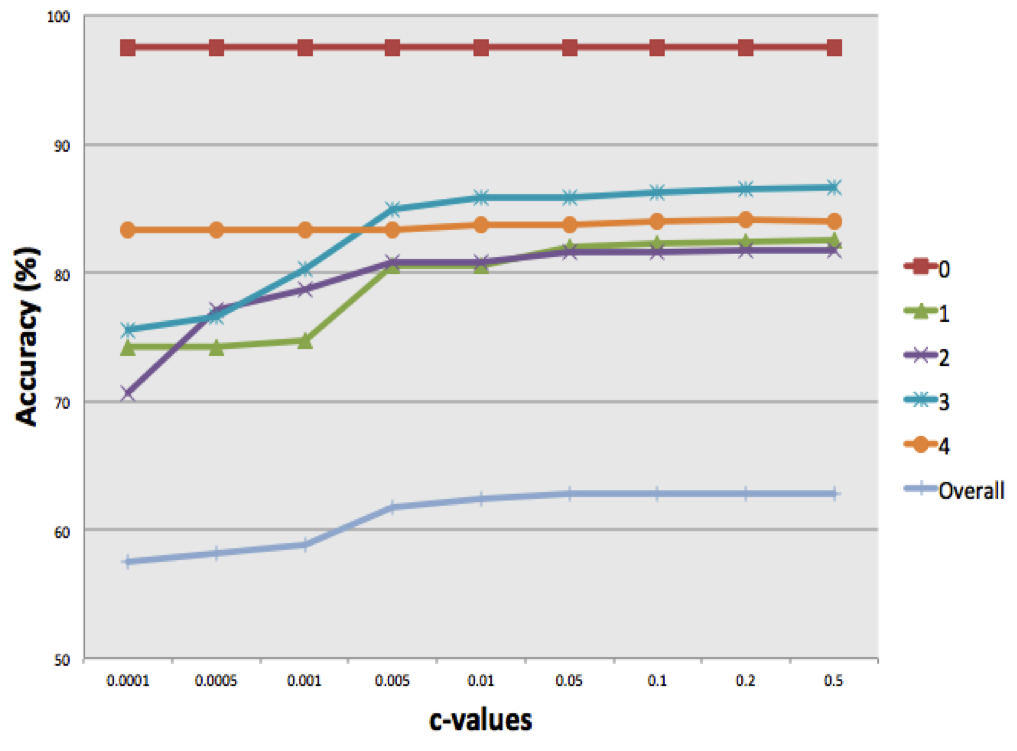
\includegraphics[width=\linewidth]{results/svmCValue}
  \caption{Accuracy vs. C-value}\label{fig:svmCValue}
\endminipage
\end{figure}


\subsubsection{Naive Bayes}
	We observed varying levels of success for different blends of n-grams. The results for all 8 possible groups of unigrams, bigrams, and trigrams can be seen in the table below. Just sticking with the conventional Naive Bayes algorithm (only using unigrams) performed fairly well. However, our intuition has told us that including bigrams and/or trigrams would lead to higher accuracies, because to infer things from sentences one often need to take context of the sentence into consideration, not just each individual word at face-value, and bigrams/trigrams introduce some level of context.

	The accuracies shown below confirm our intuition. Indeed, adding bigrams and/or trigrams into the mix lef to higher accuracies across the board (i.e. for ``Sentiment'', ``When'', and ``Kind''). And unsurprisingly, using bigrams and trigrams on ther own yielded very poor results. This is to be expected, because although certain individual words may occur frequently for certain labels (e.g. the word ``humid'' shows up frequently when the tweet is about humidity), the pairs of words within which they occur might not occur as frequently and thus not have a high class conditional probability. 

	Interestingly, using bigrams and trigrams at the same time produced slightly lower accuracies than using them individually with unigrams, but the difference in accuracy seems too low to come up with an uncontrived justification.
	
%NAIVE BAYES ACCURACY CHART
\begin{figure}[H]
\noindent\makebox[\textwidth][c]{%
\minipage{0.75\textwidth}%
  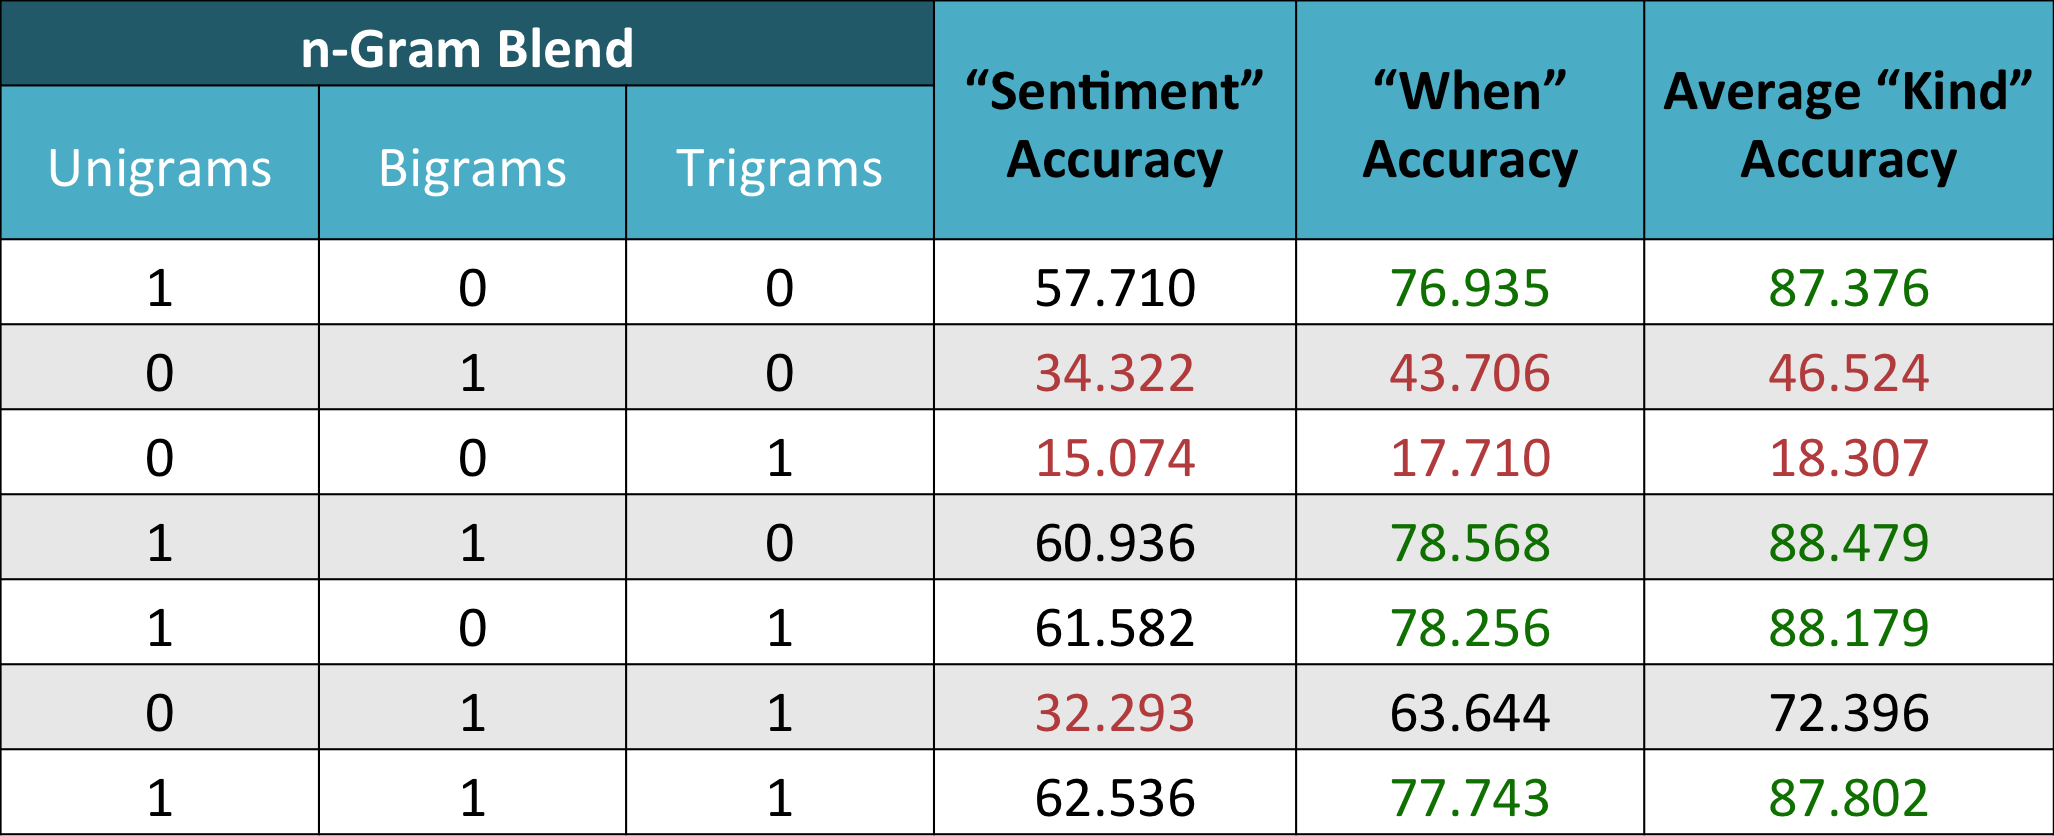
\includegraphics[width=\linewidth]{results/bayes}
  \caption{Accuracy Comparison of n-gram Blends}\label{fig:bayes}
\endminipage}
\end{figure}


\subsection{Discussion}
	All three algorithms performed significantly better than the baseline, which is a good sign right off the bat. However, certain algorithms performed better than others in some ways.

	 For sentiment, Naive Bayes displayed a higher accuracy than the other two algorithms. This makes sense because out of the three used learning methods, Naive Bayes (with the addition of bigrams and/or trigrams) is the only one that incorporates some level of sentence context. With sentiment in particular it is especially important to not just take words at face-value, but also consider the ways the neighboring words alter that word's meaning. 

	An example of this is a tweet that reads ``the weather isn't good today'', then looking at each word individually, we might say this tweet has a positive sentiment because of the presence of the word ``good'', but looking at pairs of words, the pair ``isn't good'' indicates to the learner that the user probably isn't in a positive mood. Our decision tree and SVM implementations are not as well-suited to deal with this, which explains why Naive Bayes was the best for classifying sentiment. 

	When looking at ``kind'', decision trees appeared to perform the best. This can perhaps be attributed to the fact that the presence of certain words immediately indicate what kind of weather condition the tweet is about. For example, if the word ``snowy'' is in a tweet, we can be pretty confident that one of the kinds of weather is ``snow''. Decision trees handle this well because the once the algorithm reaches a, node corresponding to the word ``snow'', it can pretty much decide then and there that weather condition is snowy and then terminate. On the other hand, Naive Bayes, for example, can notice that the word ``snow'' is in a tweet $t$, which contributes a high class conditional probabilty for the ``snowy'' weather kind, but then other words within the tweet can drag down $P(``snowy'' \mid t)$.
	
	All three algorithms did nearly-equally well at classifying ``when''. Normally, high-percentage accuracy values such as these would be quite satisfying, but our baseline was almost as high as these accuracies. That is, when we guess all ``when'' labels to be current, we get an accuracy that is only 1-2\% lower than that of our three learning algorithms. Our algorithms \emph{were} able to correctly label with other ``when'' labels, as depicted in SVM graph of when accuracies, but ultimately our data set wasn't very conducive to learning the time frame of classifying the time frame of a tweet, because our data set did not have a whole lot of variation here. 

	Below is a comparison of the three algorithms we implemented: 

%COMPARISON OF THE 3 ALGS
\begin{figure}[H]
\noindent\makebox[\textwidth][c]{%
\minipage{0.75\textwidth}%
  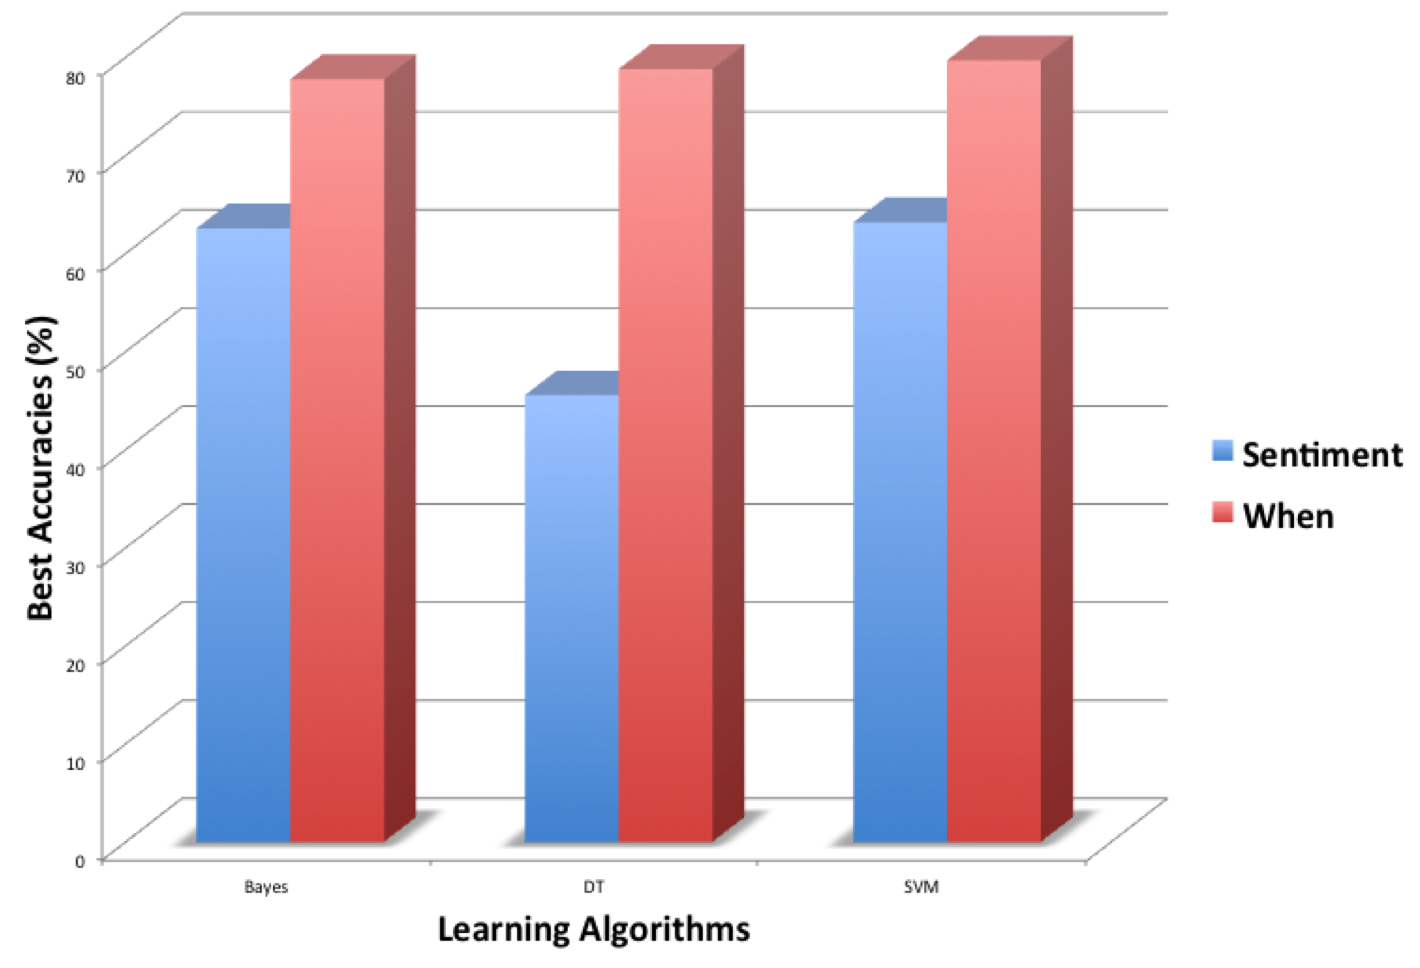
\includegraphics[width=\linewidth]{results/comparison}
  \caption{Comparison of Learning Algorithms}\label{fig:comparison}
\endminipage}
\end{figure}


	With regards to MRF, we unfortunately unable to fully implement the algorithm as specified earlier. We do, however, have a strong hunch as to what sorts of results we would have seen given the constraints of our problem. In the ideal situation, MRF would perform better than Naive Bayes, as it essentially does everything Naive Bayes can do in addition to taking account spatial/temporal dependencies. But, our formulation is not quite granular enough to expect decent accuracies. For instance, we planned to work under the assumption that the weather within each state was uniform, and the weather within one entire state is similar to that of a neighboring state. Weather varies a lot within a state, especially for large states, so we really would need to get down to the level of latitudes and longitudes (which was not available in our data set).

	Moreover, we hoped to look a small enough window of time to be able to assume that the weather within that window does not vary much. The smallest time frame we could use while still having a sufficient number of training examples was about one day -- but in practice, even one day is not small enough, because we Ithacans know better than anyone that the weather can change drastically within a day. 

	In the future, we'd like to collect more data to make this algorithm feasible, and hopefully then we can experiment with MRF and see if our high expectations are met. 



\section{Related Work}
	Out of the 4 algorithms we tried (SVM, Naive Bayes, Decision Tree and Markov Random Fields), 2 of them were Generative algorithms and 2 were Discriminative. Our Markov Random Field additionally used the conditional probabilities based on time and location of the tweets to give a similarity measure to the prediction. The training set we originally had from the Kaggle competition did not have timestamps on the tweets. This proved to be a problem for us in implementing the MRF learner, as location similarity is not enough to give an accurate classification. For instance, two particular tweets could be from the exact same location, but 6 months apart in time, therefore having different weather. 

	The research we did in bringing this project to completion allowed us to read about multiple algorithms, or modifications to existing algorithms that would give us a very robust classifier. In particular, we read about various Probabilistic Graphical Models that made the use of a ``grid-like'' arrangement of the tweets, with edges between tweets representing a dependency. The Markov Random Field algorithm we implemented was one such Probabilistic Graph Model. 

	In these models, the basic idea was that the tweets had certain independent variables, and certain dependent variables. In our situation, the independent variables were the class-conditional word probabilities (inferred from the training set word counts) and the independent variables were the location and time-based weights. Another such algorithm was the Conditional Random Field, which made the use of a similar kind of pattern recognition for structured predictions based on ``similar'' tweets. 

	The problem with most of these algorithms ended up being that they made assumptions about a sequence of observations being related. However, in our case, we had tweets that might be within the same timeframe but not related due to location differences, or vice versa. We also began with a limited dataset that did not have this vital information; and even with the Cheng-Caverlee-Lee dataset, we did not have latitudes and longitudes to introduce a proper distance-based similarity, but instead we had city and state names. Keeping in mind the constraints on our datasets, the Markov Random Field was the most appropriate to implement, using the conditional-dependencies as a Probabilistic Graphical Model.

\section{Future Work}
There are a few ways in which we look to expand upon the aforementioned algorithms:

\begin{itemize}
\item Loosening the requirement of linear separability for SVMs by incorporating kernels
\item Giving different weights to unigrams, bigrams, and trigrams in Naive Bayes
\item Adjusting weights (importance) of certain words in Naive Bayes, e.g. giving additional weight to emoticons and hashtags
\item Full implementation of MRF, performed for several different time windows and with different sets of edge matrices $T$
\item Modeling dependencies between sentiment and weather kind (e.g. if sentiment is negative, then it's more likely to be snowy than sunny)
\end{itemize}


\section{Conclusion}




%HEAT MAP
\begin{figure}[!htb]
\noindent\makebox[\textwidth][c]{%
\minipage{0.75\textwidth}%
  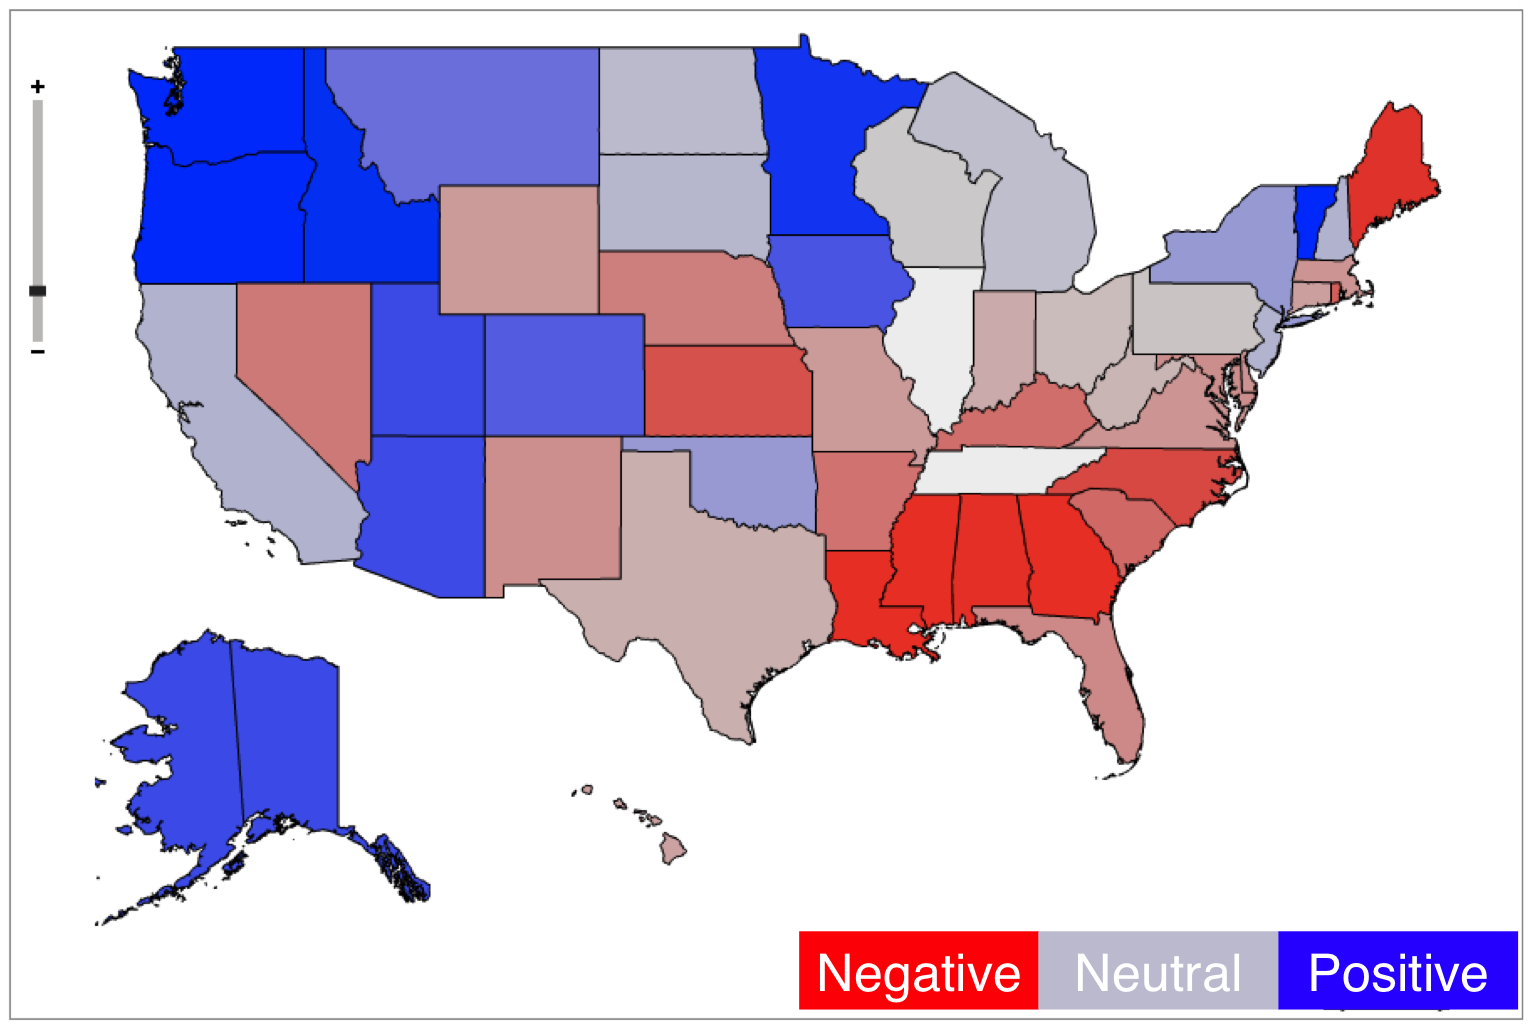
\includegraphics[width=\linewidth]{results/heatmap}
  \caption{Average ``Sentiments'' of the United States}\label{fig:heatmap}
\endminipage}
\end{figure}

\section{Appendix}
%http://www.twithawk.com/faq/stopwords used to get stopwords

%https://archive.org/details/twitter_cikm_2010 used for MRF data



\end{document}
